% Uncertainty-Aware Routing Needs an Ensemble You Do Not Have
%
% Build:  cd paper && latexmk -pdf main.tex      (or: python3 ../scripts/build_paper.py)
%
% THE PAPER CONTAINS NO TYPED NUMERALS. Every quantity below is a macro defined in
% paper/generated/numbers.tex, and every table body is a file in paper/generated/, all written by
% scripts/make_paper_tables.py from experiments/results/*/summary.json. scripts/audit_paper.py
% regenerates them and fails if anything drifted or if a numeral was typed into the prose.
\documentclass[10pt]{article}
\usepackage{tmlr}                % official TMLR style (github.com/JmlrOrg/tmlr-style-file); add [accepted] for camera-ready
\usepackage[utf8]{inputenc}
\usepackage{amsmath, amssymb}
\usepackage{booktabs}
\usepackage{graphicx}
\usepackage{microtype}
\usepackage{placeins}
\usepackage{xcolor}
\usepackage[colorlinks=true, allcolors=blue!55!black]{hyperref}

% Generated by scripts/make_paper_tables.py -- do not edit.
% Every number the paper quotes is defined here, from experiments/results/.
\newcommand{\NumChecks}{7}
\newcommand{\NumTests}{23}
\newcommand{\NumScenes}{2018}
\newcommand{\NumMembers}{12}
\newcommand{\JointStates}{81}
\newcommand{\KitchenStates}{108}
\newcommand{\FloorJ}{0.9919}
\newcommand{\FloorK}{0.7792}
\newcommand{\LogK}{1.3863}
\newcommand{\VThreeExact}{0.383812}
\newcommand{\VThreeMeas}{0.382810}
\newcommand{\RenderPairs}{682}
\newcommand{\ConfSingleLo}{0.1569}
\newcommand{\ConfSingleHi}{0.1491}
\newcommand{\ConfTrueLo}{0.0148}
\newcommand{\ConfTrueHi}{0.1491}
\newcommand{\ConfBaldLo}{0.1196}
\newcommand{\ConfBaldHi}{\ensuremath{3.7\times 10^{-19}}}
\newcommand{\ConfRiseJ}{10.0}
\newcommand{\ConfRiseK}{9.5}
\newcommand{\ConfOverstate}{8.1}
\newcommand{\ConfCross}{0.5}
\newcommand{\RoutBaldRhoZero}{\ensuremath{+0.114}}
\newcommand{\RoutBaldRhoHigh}{\ensuremath{-0.053}}
\newcommand{\RoutBaldRhoOne}{\ensuremath{-0.009}}
\newcommand{\RoutSkillBaldRhoZero}{\ensuremath{+0.09}}
\newcommand{\RoutSkillBaldRhoHigh}{\ensuremath{-0.15}}
\newcommand{\DecAleaTrue}{0.9897}
\newcommand{\DecAleaHatLo}{0.65}
\newcommand{\DecAleaHatHi}{1.39}
\newcommand{\DecTempHalfHat}{0.65}
\newcommand{\DecTempTwoHat}{1.23}
\newcommand{\DecAcc}{0.575}
\newcommand{\DecMarginalEpiTrue}{0.386}
\newcommand{\RoutTotalLo}{\ensuremath{+0.336}}
\newcommand{\RoutTotalHi}{\ensuremath{-0.590}}
\newcommand{\RoutBaldLo}{\ensuremath{+0.294}}
\newcommand{\RoutBaldHi}{\ensuremath{-0.223}}
\newcommand{\RoutFloorLo}{0.72}
\newcommand{\RoutFloorHi}{1.33}
\newcommand{\RoutSkillTotalHi}{\ensuremath{-0.61}}
\newcommand{\MechJMissEvLo}{\ensuremath{+0.158}}
\newcommand{\MechJMissEvHi}{\ensuremath{+0.043}}
\newcommand{\BaldJMissEvLo}{\ensuremath{+nan}}
\newcommand{\BaldJMissEvHi}{\ensuremath{+nan}}
\newcommand{\MechJNoiseLo}{\ensuremath{+0.375}}
\newcommand{\MechJNoiseHi}{\ensuremath{-0.613}}
\newcommand{\BaldJNoiseLo}{\ensuremath{+0.327}}
\newcommand{\BaldJNoiseHi}{\ensuremath{-0.236}}
\newcommand{\MechJOverLo}{\ensuremath{-0.443}}
\newcommand{\MechJOverHi}{\ensuremath{-0.992}}
\newcommand{\BaldJOverLo}{\ensuremath{+nan}}
\newcommand{\BaldJOverHi}{\ensuremath{+nan}}
\newcommand{\MechJUnderLo}{\ensuremath{-0.307}}
\newcommand{\MechJUnderHi}{\ensuremath{-0.978}}
\newcommand{\BaldJUnderLo}{\ensuremath{+nan}}
\newcommand{\BaldJUnderHi}{\ensuremath{+nan}}
\newcommand{\MechJEnsLo}{\ensuremath{-0.277}}
\newcommand{\MechJEnsHi}{\ensuremath{-0.460}}
\newcommand{\BaldJEnsLo}{\ensuremath{+0.557}}
\newcommand{\BaldJEnsHi}{\ensuremath{+0.663}}
\newcommand{\MechJMixedLo}{\ensuremath{+0.405}}
\newcommand{\MechJMixedHi}{\ensuremath{-0.494}}
\newcommand{\BaldJMixedLo}{\ensuremath{+0.354}}
\newcommand{\BaldJMixedHi}{\ensuremath{-0.163}}
\newcommand{\MechKMissEvLo}{\ensuremath{+0.190}}
\newcommand{\MechKMissEvHi}{\ensuremath{+0.168}}
\newcommand{\BaldKMissEvLo}{\ensuremath{+nan}}
\newcommand{\BaldKMissEvHi}{\ensuremath{+nan}}
\newcommand{\MechKNoiseLo}{\ensuremath{+0.306}}
\newcommand{\MechKNoiseHi}{\ensuremath{-0.574}}
\newcommand{\BaldKNoiseLo}{\ensuremath{+0.311}}
\newcommand{\BaldKNoiseHi}{\ensuremath{-0.238}}
\newcommand{\MechKOverLo}{\ensuremath{-0.223}}
\newcommand{\MechKOverHi}{\ensuremath{-1.000}}
\newcommand{\BaldKOverLo}{\ensuremath{+nan}}
\newcommand{\BaldKOverHi}{\ensuremath{+nan}}
\newcommand{\MechKUnderLo}{\ensuremath{-0.722}}
\newcommand{\MechKUnderHi}{\ensuremath{-0.997}}
\newcommand{\BaldKUnderLo}{\ensuremath{+nan}}
\newcommand{\BaldKUnderHi}{\ensuremath{+nan}}
\newcommand{\MechKEnsLo}{\ensuremath{-0.441}}
\newcommand{\MechKEnsHi}{\ensuremath{-0.624}}
\newcommand{\BaldKEnsLo}{\ensuremath{+0.819}}
\newcommand{\BaldKEnsHi}{\ensuremath{+0.843}}
\newcommand{\MechKMixedLo}{\ensuremath{+0.306}}
\newcommand{\MechKMixedHi}{\ensuremath{-0.495}}
\newcommand{\BaldKMixedLo}{\ensuremath{+0.239}}
\newcommand{\BaldKMixedHi}{\ensuremath{-0.200}}
\newcommand{\PreShareLo}{92\%}
\newcommand{\PreShareHi}{97\%}
\newcommand{\PreJModelOne}{\ensuremath{-0.189}}
\newcommand{\PreJPrefixOne}{\ensuremath{+0.151}}
\newcommand{\PreJModelTwo}{\ensuremath{+0.001}}
\newcommand{\PreJPrefixTwo}{\ensuremath{+0.135}}
\newcommand{\PreJModelFour}{\ensuremath{+0.084}}
\newcommand{\PreJPrefixFour}{\ensuremath{+0.117}}
\newcommand{\PreJModelEight}{\ensuremath{+0.127}}
\newcommand{\PreJPrefixEight}{\ensuremath{+0.070}}
\newcommand{\PreKModelOne}{\ensuremath{-0.490}}
\newcommand{\PreKPrefixOne}{\ensuremath{+0.059}}
\newcommand{\PreKModelTwo}{\ensuremath{-0.346}}
\newcommand{\PreKPrefixTwo}{\ensuremath{+0.052}}
\newcommand{\PreKModelFour}{\ensuremath{-0.220}}
\newcommand{\PreKPrefixFour}{\ensuremath{+0.083}}
\newcommand{\PreKModelEight}{\ensuremath{-0.133}}
\newcommand{\PreKPrefixEight}{\ensuremath{+0.060}}
\newcommand{\PreJFloorOne}{1.2122}
\newcommand{\PreJFloorLast}{0.9932}
\newcommand{\RobSeeds}{5}
\newcommand{\RobBoot}{1000}
\newcommand{\RobMechCells}{24}
\newcommand{\RobMechStable}{24}
\newcommand{\RobRiseLo}{9.8}
\newcommand{\RobRiseHi}{10.6}
\newcommand{\RobBaldEnsLo}{\ensuremath{+0.563}}
\newcommand{\RobBaldEnsHi}{\ensuremath{+0.840}}
\newcommand{\RobBaldEnsSd}{0.012}
\newcommand{\RobPreShareLo}{92\%}
\newcommand{\RobPreShareHi}{98\%}
\newcommand{\RobPreCells}{8}
\newcommand{\RobPrePositive}{8}
\newcommand{\RobPreModel}{7}
\newcommand{\RobOverHiSd}{0.001}
\newcommand{\RobOverLoCI}{[\ensuremath{-0.485}, \ensuremath{-0.398}]}
\newcommand{\RobEnsHiCI}{[\ensuremath{+0.630}, \ensuremath{+0.694}]}
\newcommand{\RobMissEvHiCI}{[\ensuremath{-0.001}, \ensuremath{+0.086}]}
\newcommand{\RobPreJTwoMean}{\ensuremath{-0.014}}
\newcommand{\RobPreJTwoSd}{0.020}


\newcommand{\Pstar}{P^{*}}
\newcommand{\KL}[2]{\mathrm{KL}(#1\,\|\,#2)}

\title{Uncertainty-Aware Routing Needs an Ensemble You Do Not Have}
\author{\name Anonymous authors}
% Non-anonymous form: replace the line above with the author block the venue asks for.

\begin{document}
\maketitle

\begin{abstract}
Escalating a query to an expensive model pays off only when the cheap model's error is
\emph{reducible}, so uncertainty-aware routers decompose predictive uncertainty and route on the
reducible part. Two 2026 results establish the pieces this rests on: the mutual-information
estimate of epistemic uncertainty is not the reducible kind, and the irreducible term cancels from
the escalation decision. Both assume the estimator one would like --- independently seeded
ensemble members, or multiple independent annotations per input. We ask what the estimator you can
actually build does instead, in a synthetic video-forecasting world where the true conditional
$\Pstar$ is exact in closed form, so every estimate can be compared against the quantity it claims
to estimate. (i) As members go from independent to identical at fixed per-member error, the
ensemble's true error rises $\ConfRiseJ\times$ while its estimate falls to zero; they cross near
$\rho=\ConfCross$, and the estimator's advantage over random routing is gone by $\rho=0.75$.
(ii) Whether confidence routing decays or inverts below random is decided by \emph{why} the cheap
model is worse: benign under missing evidence, catastrophic under miscalibration, floor-invariant
where the estimate is well-posed. (iii) Video has a second lever, and
\RobPreShareLo--\RobPreShareHi{} of the gain from extending the observed prefix is exactly the term
that cancels from model escalation. Everything reproduces over \RobSeeds{} seeds and two
structurally different worlds. No vision-language model was run, and nothing here is evidence
about real video.
\end{abstract}

\section{Introduction}

A forecaster sees a prefix of video and reports a distribution over what happens next. When the
answer is uncertain, a deployed system can spend to improve it --- escalate to a larger model, whose
cost-quality frontier is by now well characterised \citep{bouchard2026escalation} --- but only if
the uncertainty is the kind that spending removes. For a forecast $Q$ on a scene whose true
conditional is $\Pstar$, the expected log loss splits exactly:
%
\begin{equation}
\mathbb{E}_{y\sim \Pstar}\!\left[-\log Q(y)\right]
  \;=\; \underbrace{H(\Pstar)}_{\text{irreducible}} \;+\; \underbrace{\KL{\Pstar}{Q}}_{\text{the forecaster's}}
\label{eq:split}
\end{equation}
%
This is an identity. $H(\Pstar)$ is a property of the world and the prefix: no forecaster reduces
it and every forecaster pays it. $\KL{\Pstar}{Q}$ is a property of the forecaster, zero exactly at
Bayes-optimality, and it is the entire quantity a better model could recover. Escalating one scene
from a cheap forecaster $Q_c$ to an expensive $Q_e$ therefore changes expected loss by
%
\begin{equation}
\big[H(\Pstar) + \KL{\Pstar}{Q_c}\big] - \big[H(\Pstar) + \KL{\Pstar}{Q_e}\big]
  \;=\; \KL{\Pstar}{Q_c} - \KL{\Pstar}{Q_e}
\label{eq:gain}
\end{equation}
%
The irreducible term cancels exactly. But the total predictive entropy $H(\bar Q)$ that
confidence-based routing ranks by \emph{contains} that term, and is often dominated by it.

\paragraph{What is already established, and is not claimed here.}
\citet{young2026epistemic} proves that the standard definition of epistemic uncertainty and its
standard mutual-information measure \citep{houlsby2011bayesian, depeweg2018decomposition},
estimated in practice from an ensemble \citep{lakshminarayanan2017simple}, are
extensionally inconsistent, and that ensemble disagreement ``collapses to zero beneath a positive
truth under consistent training''. \citet{peale2026flexible} state the cancellation in
\eqref{eq:gain} in their introduction, build a router that decomposes total uncertainty via
higher-order predictors \citep{ahdritz2025provable}, and show total-uncertainty routing
underperforming a pointwise-optimal policy. So the inequality between disagreement and forecaster
error, the cancellation, and the failure of total-uncertainty routing are \emph{not}
contributions of this paper. We take them as the setting.

\paragraph{What neither covers.}
Both assume the estimator one would like. \citet{young2026epistemic} assumes independently seeded
members; \citet{peale2026flexible} require multiple independent annotations per input plus a
higher-order calibration guarantee. The practical substitute is an ensemble of similarly
pre-trained models, or repeated calls to one model, whose errors are correlated by construction.
That correlation is the free parameter neither paper sweeps, and it is the one a deployment does
not get to choose. Relatedly, \citet{kirsch2024implicit} reports epistemic estimates collapsing as
model \emph{complexity} rises, by implicit ensembling --- a different cause, and without a routing
experiment or a known ground-truth epistemic error to compare against.

\paragraph{Contributions.} Three, each measured against a closed-form $\Pstar$, against an explicit
random-routing baseline, in two structurally different worlds: (i) a \emph{$\rho$-parameterised}
link from ensemble-member correlation to routing performance, in which the estimate and the error
it stands in for cross (\S\ref{sec:confound}); (ii) a \emph{mechanism map}, in which the cause of
the cheap model's deficit --- not the irreducible floor --- decides whether confidence routing
decays or inverts (\S\ref{sec:mechanisms}); and (iii) the \emph{prefix lever}, which is specific to
video and whose gain is almost entirely the term that cancels from model escalation
(\S\ref{sec:prefix}). Everything is re-run across seeds and bootstrapped
(\S\ref{sec:robustness}). The world is synthetic, no vision-language model was called and no video
corpus was used; \S\ref{sec:limits} says what that costs.

\section{An instrument in which the floor is known}
\label{sec:instrument}

$\Pstar$ is not observable on real video: nobody knows the true distribution of the future given a
clip, so $H(\Pstar)$ there can only be assumed. Every empirical claim about aleatoric uncertainty
on real video is therefore a claim about an estimator whose target is unavailable for comparison.
We work where the target exists.

A scene carries latent cues $z$ with finite alphabets and independent priors. The outcome is drawn
from $P(y\mid z)$, with logits linear in the cues (world \textsc{junction}) or carrying pairwise
interactions (world \textsc{kitchen}), softened by a temperature $\tau$. A prefix reveals a subset
of the cues, recorded by an observability mask $m$ drawn independently of $z$, so the best any
forecaster can do is $\Pstar(y \mid z_m) = \sum_{z_h} P(z_h)\,P(y \mid z_m, z_h)$ --- an exact
finite sum over $\JointStates$ joint cue states and $16$ masks. $\tau$ is the only knob on the
irreducible floor, which runs $\RoutFloorLo$ to $\RoutFloorHi$ nats against a ceiling of
$\log 4 = \LogK$; prefix length is a second, used in \S\ref{sec:prefix}.

Forecasters are chosen so their behaviour is known in closed form before they run: Bayes-optimal
(epistemic exactly zero), uniform (expected loss exactly $\log K$), marginal (excess loss exactly
$I(y; z_m)$), partial-evidence, tempered, logit-noise with an ensemble-correlation parameter
$\rho$, and cue-dropout. That is what makes the instrument checkable rather than merely plausible:
\NumChecks{} validation checks, each with an answer fixed by the mathematics rather than by a
previous run, pass in \emph{both} worlds --- Bayes-optimal epistemic error $0$ exactly, the
marginal forecaster's excess loss $\VThreeMeas$ against an enumerated $\VThreeExact$, and an
evidence ladder matching every rung of its closed form (Appendix~\ref{app:instrument}).

\paragraph{Metric.} We report the Spearman correlation between a policy's score and the true
escalation gain of \eqref{eq:gain}, per scene: it is zero when a policy carries no signal, and a
\emph{negative} value has a deployment meaning --- the policy is worse than routing at random,
spending the budget on the scenes with the least recoverable error. Budgeted curves normalised so
random scores $0$ and the oracle $1$ are in Appendix~\ref{app:curves} and agree on every sign
below. Every number comes from $\NumScenes$ held-out scenes and $\NumMembers$-member ensembles.

\section{Correlated members: the estimate and the error move in opposite directions}
\label{sec:confound}

The probe holds each member's own marginal noise scale fixed while sweeping the fraction $\rho$ of
the logit perturbation that members share. A single member's error therefore does not change with
$\rho$; only the ensemble's ability to see it does. That invariance is what makes the sweep
readable, and it is asserted by a test.

\begin{table}[t]
\centering
\small
\caption{As ensemble members go from independent to identical at fixed per-member error
(\textsc{junction}, $\tau{=}0.9$). Column 1 is the control. The deployed ensemble's true error
rises $\ConfRiseJ\times$; the estimate of it falls to zero. They cross near $\rho=\ConfCross$.}
\label{tab:confound}
\begin{tabular}{lccc}
\toprule
$\rho$ & one member's error & ensemble's \textbf{true} error $\KL{\Pstar}{\bar Q}$ & ensemble's \textbf{estimate} (BALD) \\
\midrule
% Generated by scripts/make_paper_tables.py -- do not edit.
0.00 & 0.1569 & 0.0148 & 0.1196 \\
0.25 & 0.1569 & 0.0432 & 0.0907 \\
0.50 & 0.1558 & 0.0750 & 0.0614 \\
0.75 & 0.1540 & 0.1102 & 0.0313 \\
0.90 & 0.1521 & 0.1330 & 0.0127 \\
1.00 & 0.1491 & 0.1491 & $<10^{-18}$
 \\
\bottomrule
\end{tabular}
\end{table}

Table~\ref{tab:confound} reads in three parts. A single member's error is flat
($\ConfSingleLo \to \ConfSingleHi$). The deployed ensemble's \emph{true} error rises
$\ConfRiseJ\times$ ($\ConfTrueLo \to \ConfTrueHi$), because averaging cancels only the error the
members do not share. The \emph{estimate} falls to $\ConfBaldHi$, because it measures disagreement
and identical members do not disagree. At $\rho=0$ the estimate overstates the ensemble's error by
$\ConfOverstate\times$; at $\rho=1$ it reports zero for an ensemble carrying $\ConfTrueHi$ nats of
recoverable error. The two quantities cross near $\rho=\ConfCross$, so there is no correlation
level at which the estimate is merely conservative.

\paragraph{What that costs a router.} At a fixed world, ranking scenes by the estimate correlates
$\RoutBaldRhoZero$ with the true gain at $\rho=0$ and $\RoutBaldRhoHigh$ at $\rho=0.75$; its
budgeted skill against random goes $\RoutSkillBaldRhoZero \to \RoutSkillBaldRhoHigh$. The
advantage the estimator exists to provide is gone --- and below random --- before members are
anywhere near identical. A single deterministic model is the $\rho=1$ case in its most extreme and
most common form: the estimate is identically zero and induces no ranking at all, including for a
forecaster that ignores the prefix entirely and carries $\DecMarginalEpiTrue$ nats of recoverable
error.

The aleatoric half of the same estimate fails in the mirror-image way: the true irreducible term is
$\DecAleaTrue$ nats for every forecaster, as \eqref{eq:split} requires, while the estimate of it
swings from $\DecAleaHatLo$ to $\DecAleaHatHi$ with the forecaster's confidence --- two forecasters
with identical accuracy and identical true irreducible uncertainty report $\DecTempHalfHat$ and
$\DecTempTwoHat$ (Appendix~\ref{app:decomposition}).

\section{Whether confidence routing inverts depends on why the cheap model is worse}
\label{sec:mechanisms}

Sweeping the floor with one cheap/expensive pair invites the reading that the floor is the whole
story. It is not. Table~\ref{tab:mechanisms} fixes the pair's \emph{cause} and sweeps the floor,
with a random baseline at zero by construction.

\begin{table}[t]
\centering
\small
\caption{$\mathrm{corr}(\text{score}, \text{true gain})$ in \textsc{junction}, by why the cheap
forecaster is worse; negative is worse than routing at random. \emph{n/a} marks a configuration
where the estimate does not exist rather than being small: a single deterministic forecaster has no
ensemble spread, so BALD is identically zero and induces no ranking. The irreducible floor
$\mathbb{E}[H(\Pstar)]$ runs $\RoutFloorLo \to \RoutFloorHi$ nats across the columns.}
\label{tab:mechanisms}
\begin{tabular}{lccccccc}
\toprule
& \multicolumn{5}{c}{ranking by total uncertainty, $\tau =$} & \multicolumn{2}{c}{BALD} \\
\cmidrule(lr){2-6}\cmidrule(lr){7-8}
why the cheap model is worse & % Generated by scripts/make_paper_tables.py -- do not edit.
0.35 & 0.70 & 1.30 & 2.00 & 3.50
 & $\tau{=}0.35$ & $\tau{=}3.5$ \\
\midrule
% Generated by scripts/make_paper_tables.py -- do not edit.
missing evidence & \ensuremath{+0.16} & \ensuremath{+0.13} & \ensuremath{+0.05} & \ensuremath{+0.08} & \ensuremath{+0.04} & n/a & n/a \\
injected noise & \ensuremath{+0.37} & \ensuremath{+0.24} & \ensuremath{-0.01} & \ensuremath{-0.25} & \ensuremath{-0.61} & \ensuremath{+0.33} & \ensuremath{-0.24} \\
overconfidence ($T{=}0.4$) & \ensuremath{-0.44} & \ensuremath{-0.75} & \ensuremath{-0.97} & \ensuremath{-1.00} & \ensuremath{-0.99} & n/a & n/a \\
underconfidence ($T{=}2.5$) & \ensuremath{-0.31} & \ensuremath{-0.72} & \ensuremath{-0.93} & \ensuremath{-0.97} & \ensuremath{-0.98} & n/a & n/a \\
evidence ensemble & \ensuremath{-0.28} & \ensuremath{-0.33} & \ensuremath{-0.45} & \ensuremath{-0.46} & \ensuremath{-0.46} & \ensuremath{+0.56} & \ensuremath{+0.66} \\
mixed & \ensuremath{+0.41} & \ensuremath{+0.29} & \ensuremath{+0.09} & \ensuremath{-0.10} & \ensuremath{-0.49} & \ensuremath{+0.35} & \ensuremath{-0.16}
 \\
\bottomrule
\end{tabular}
\end{table}

\textbf{Missing evidence is benign.} A model that cannot see a cue is honestly uncertain, and that
is also where a better model gains. The correlation decays toward zero
($\MechJMissEvLo \to \MechJMissEvHi$) but never inverts --- literally toward zero, in that the
high-floor end has a bootstrap interval of $\RobMissEvHiCI$, so the honest reading there is
``no signal'' rather than ``a little signal''.

\textbf{Miscalibration is catastrophic, and it inverts at every floor.} An overconfident model's
entropy is lowest exactly where it is most wrong, so ranking by entropy systematically selects the
scenes it already handles: $\MechJOverLo \to \MechJOverHi$. Underconfidence is nearly as bad
($\MechJUnderLo \to \MechJUnderHi$). This is the case that matters outside a synthetic world,
because overconfidence is the documented failure mode of neural classifiers
\citep{guo2017calibration} rather than a hypothetical one. \citet{xia2025label} document the same
direction for label smoothing in selective classification; what the controlled floor adds is that
the inversion is not a property of the regulariser but of the confidence--error relationship, and
that it deepens monotonically as the irreducible floor rises.

\textbf{Where the estimate is well-posed, it works, and it is floor-invariant.} With members that
disagree because evidence is missing --- errors independent by construction --- BALD scores
$\BaldJEnsLo \to \BaldJEnsHi$ and does not degrade at all as the floor rises, while total
uncertainty is worse than random everywhere in the same setting
($\MechJEnsLo \to \MechJEnsHi$); in the non-additive world it is stronger still
($\BaldKEnsLo \to \BaldKEnsHi$). This is the positive result, and it is what makes the negative
ones worth reporting: the distinction in \eqref{eq:split} is real and actionable, and the whole
difficulty is in estimating it.

The mechanism is explicable rather than mysterious: high predictive entropy selects scenes where
the ensemble has hedged toward uniform, hedging toward uniform is close to optimal precisely when
the world is uncertain, and those are the scenes with the least recoverable error.
\citet{peale2026flexible} name an adjacent condition --- a benefit ``whenever reducible and
irreducible uncertainty are not too correlated'' --- on a different axis: theirs is the correlation
between the two terms, ours is the cause of the deficit, which a practitioner can diagnose directly
by measuring calibration.

\section{Video has a second lever, and it is made of the term that cancels}
\label{sec:prefix}

An uncertain forecast admits two responses: spend on the model, or spend on the evidence. The
second is available in video and not in image classification. It does not obey \eqref{eq:gain},
because a longer prefix changes $\Pstar$ itself:
%
\begin{equation}
\text{gain(extend prefix } L \to L')
  = \big[H(\Pstar_L) + \KL{\Pstar_L}{Q}\big] - \big[H(\Pstar_{L'}) + \KL{\Pstar_{L'}}{Q}\big],
\label{eq:prefix}
\end{equation}
%
whose leading term is $H(\Pstar_L) - H(\Pstar_{L'})$ --- exactly the quantity that cancels from
model escalation. Masks are nested across lengths, since evidence does not disappear as one keeps
watching, and the floor is enumerated rather than sampled at every length
($\PreJFloorOne \to \PreJFloorLast$ nats as $L$ goes $1 \to 32$).

\begin{table}[t]
\centering
\small
\caption{The two decisions are driven by almost disjoint quantities. Share is the fraction of the
mean prefix-extension gain that is $\Delta H(\Pstar)$; the correlations are
$\mathrm{corr}(\text{total uncertainty}, \text{gain})$ for each of the two available actions.}
\label{tab:prefix}
\begin{tabular}{lcccccc}
\toprule
& \multicolumn{3}{c}{\textsc{junction} (additive evidence)} & \multicolumn{3}{c}{\textsc{kitchen} (non-additive)} \\
\cmidrule(lr){2-4}\cmidrule(lr){5-7}
prefix $L$ & $\Delta H(\Pstar)$ share & $\to$ model & $\to$ prefix & $\Delta H(\Pstar)$ share & $\to$ model & $\to$ prefix \\
\midrule
% Generated by scripts/make_paper_tables.py -- do not edit.
$1\!\to\!2$ & 94\% & \ensuremath{-0.189} & \ensuremath{+0.151} & 97\% & \ensuremath{-0.490} & \ensuremath{+0.059} \\
$2\!\to\!4$ & 94\% & \ensuremath{+0.001} & \ensuremath{+0.135} & 93\% & \ensuremath{-0.346} & \ensuremath{+0.052} \\
$4\!\to\!8$ & 95\% & \ensuremath{+0.084} & \ensuremath{+0.117} & 96\% & \ensuremath{-0.220} & \ensuremath{+0.083} \\
$8\!\to\!16$ & 92\% & \ensuremath{+0.127} & \ensuremath{+0.070} & 97\% & \ensuremath{-0.133} & \ensuremath{+0.060}
 \\
\bottomrule
\end{tabular}
\end{table}

The robust part is the share: \PreShareLo--\PreShareHi{} of the prefix-extension gain is the term
that cancels entirely from model escalation, at every length in both worlds. The two decisions are
therefore driven by almost disjoint quantities, and a system that ranks both by one confidence
score is answering the wrong question about one of them.

Whether the two correlations have \emph{opposite signs} depends on the world, and the honest
version is the narrower one. In \textsc{kitchen} they do at every length: total uncertainty
correlates $\PreKModelOne \to \PreKModelEight$ with the model decision and
$\PreKPrefixOne \to \PreKPrefixEight$ with the prefix decision throughout. In \textsc{junction} the
opposition holds only at the shortest prefix ($\PreJModelOne$ against $\PreJPrefixOne$); by
$4\to8$ the model correlation has turned positive. Short prefixes with interacting cues are the
regime video forecasting operates in, and it is where the opposition is robust; the additive world
is where it is not. Prior work on video anticipation under ambiguity treats the prediction
\emph{horizon} as the axis \citep{farha2019uncertainty}; the observation prefix is a different
lever, and the non-cancellation in \eqref{eq:prefix} is what makes it a different decision.

\section{Robustness}
\label{sec:robustness}

Every claim above is a claim about a sign, and a sign from one run is not yet a claim. We re-ran
all three families over \RobSeeds{} seeds --- re-drawing the scenes \emph{and} the forecasters'
noise streams --- and separately bootstrapped the published run with \RobBoot{} resamples of the
scenes, which keeps seed-to-seed variation apart from the precision of a single reported figure
(Appendix~\ref{app:robustness}) --- and for one cell the seed spread lies outside that run's
bootstrap interval, which is the reason to report both rather than either.
\RobMechStable{} of \RobMechCells{} (world, mechanism, floor) cells keep their published sign at
every seed. The rise in the ensemble's true error as
$\rho: 0 \to 1$ is $\RobRiseLo$--$\RobRiseHi\times$ across seeds and worlds. BALD on the well-posed
ensemble averages $\RobBaldEnsLo$ to $\RobBaldEnsHi$ with a seed standard deviation of at most
$\RobBaldEnsSd$ and a bootstrap interval of $\RobEnsHiCI$ at the high floor; the overconfidence
inversion at the low floor sits in $\RobOverLoCI$. The prefix share is
\RobPreShareLo--\RobPreShareHi{} over every seed, world and length, and the prefix-decision
correlation stays positive in \RobPrePositive{} of \RobPreCells{} cells. One cell is not
sign-stable and should not be read as a sign: the model-decision correlation keeps its sign in only
\RobPreModel{} of \RobPreCells{}, the exception being \textsc{junction} $2\to4$, whose published
value $\PreJModelTwo$ is indistinguishable from zero --- the cell \S\ref{sec:prefix} already
excludes.

\section{What this is not evidence about}
\label{sec:limits}

\textbf{The world is synthetic, and that is not incidental.} $\Pstar$ exists here because we built
it, so nothing above is evidence about any real corpus. That it transfers is an argument and not a
measurement: the estimators under test are the deployed ones, so showing what they do where the
truth is known is informative about what they do where it is not. A reader may decline the
argument, and should then read every claim here as a claim about estimators only.
\textbf{$\rho$ is a knob, not a measurement:} we show what member correlation costs a router, not
the $\rho$ of any real ensemble, and whether repeated calls to one model form a high-$\rho$
ensemble is an assumption --- made more plausible by the removal of temperature controls from
current model APIs, but not established here. \textbf{No vision-language model was called:} the arm
is implemented, prompted, cached and costed at roughly one dollar, and no credential existed on
the machine to run it. It is the only setting in which a real model could be handed a true
$\KL{\Pstar}{Q}$, and its three predictions are recorded, falsifiable and untested.

\section{Conclusion}

The reducible/irreducible distinction is real and actionable: where the estimate is well-posed it
ranks escalation candidates at $\BaldJEnsLo$ to $\BaldKEnsHi$ and does not care how uncertain the
world is. The difficulty is entirely in estimating it, and the regime where the estimate inverts
against the truth --- members that share their errors --- is the regime a deployment is in.
Confidence routing's failure, meanwhile, is not a fact about confidence but about the cheap model's
calibration, which is diagnosable in advance; and video's second lever is made almost entirely of
the term that cancels from the first, so one score cannot serve both.

\small
\bibliographystyle{tmlr}
\bibliography{refs}

\normalsize
\appendix
\newpage

\section{The instrument, and the two worlds}
\label{app:instrument}

% Generated by scripts/make_paper_tables.py -- do not edit.
Every result in the paper is measured in two worlds that differ on every axis that
could plausibly matter, so that a finding which depends on the construction can be told from one
that does not. \textsc{kitchen} is the important one: its evidence is \emph{non-additive}, so
losing a cue can be catastrophic rather than gradual, which is the structure most likely to break
a mechanism map built on gradual evidence loss. Cue visibilities are deliberately spread rather
than uniform --- if every cue were equally visible the observability mask would carry no
information and every scene would sit at the same irreducible floor, which is the degenerate case
a routing experiment must avoid.

\begin{table}[h]
\centering
\small
\caption{The two worlds. Only the second admits interactions between cues, and the instrument's
checks are world-independent by construction rather than by configuration.}
\begin{tabular}{lcc}
\toprule
& \textsc{junction} & \textsc{kitchen} \\
\midrule
outcomes & 4 & 3 \\
cues & 4 & 5 \\
cue alphabets & uniformly ternary & mixed binary and ternary \\
symmetry & left/right mirrored & none \\
evidence & \textbf{additive} (linear in the cues) & \textbf{non-additive} (pairwise) \\
joint cue states & \JointStates & \KitchenStates \\
irreducible floor at the default $\tau$ & \FloorJ{} nats & \FloorK{} nats \\
validation checks passed & \NumChecks/\NumChecks & \NumChecks/\NumChecks \\
\bottomrule
\end{tabular}
\end{table}


\begin{table}[h]
\centering
\small
\caption{The validation checks. Each expectation was fixed by the mathematics before the check
ran, and every check is world-independent by construction --- which is tested rather than asserted
by running them in the second world, where they also pass.}
\label{tab:validation}
\begin{tabular}{@{}lp{0.27\textwidth}p{0.29\textwidth}p{0.27\textwidth}@{}}
\toprule
& claim & expected & measured \\
\midrule
% Generated by scripts/make_paper_tables.py -- do not edit.
V1 & Bayes-optimal forecaster has zero epistemic uncertainty & max KL(P*$\|$Q) = 0 exactly & max = 0.000e+00 \\
V2 & Uniform forecaster scores log K on every scene & expected NLL = log 4 = 1.386294 exactly & max deviation = 4.441e-16 \\
V3 & Marginal forecaster's excess loss equals I(y; z\_m) & I(y; z\_m) = 0.383812 nats (exact) & 0.382810 $\pm$ 0.014659 (3 sem) \\
V4 & Expected epistemic error is monotone in the cues used, and matches closed form & ladder non-decreasing; every rung within 3 sem of its enumerated value & monotone=True; 5/5 rungs match \\
V5 & Aleatoric floor is non-increasing in prefix length & every successive difference $\leq$ 0 & max increase = -1.014e-02 \\
V6 & As members correlate, the estimate and the true error move in opposite directions & single-member error flat; KL(P*$\|$Qbar) rises monotonically; BALD falls monotonically to 0 & single 0.1569$\to$0.1491; true 0.0148$\to$0.1491 (10.0x); BALD 0.1196$\to$3.75e-19 \\
V7 & Oracle routing dominates every policy at every budget & no policy achieves lower loss than the oracle at any budget & largest violation = 0.000e+00
 \\
\bottomrule
\end{tabular}
\end{table}

A renderer exists so that the vision-language arm would be a real experiment rather than a
description of one; it is not used by any measurement in this paper. Its contract is that a cue the
mask hides must not be recoverable from the pixels, which is verified on $\RenderPairs$ scene pairs
differing only in a hidden cue: maximum pixel difference exactly zero.

\FloatBarrier
\section{The full decomposition table}
\label{app:decomposition}

\begin{table}[h]
\centering
\small
\caption{Both decompositions side by side, \textsc{junction}, $\tau{=}0.9$. The
\textbf{true} irreducible column is constant, as \eqref{eq:split} requires. The \textbf{estimated}
column (bold) is not: it tracks the forecaster's confidence. The estimated epistemic column is
exactly zero for every deterministic forecaster, including one whose true epistemic error is the
largest in the table among forecasters that read the prefix at all.}
\label{tab:decomposition}
\begin{tabular}{lccccc}
\toprule
forecaster & irred.\ true & irred.\ \textbf{est.} & epist.\ true & epist.\ est. & acc. \\
\midrule
% Generated by scripts/make_paper_tables.py -- do not edit.
Bayes-optimal & 0.9897 & \textbf{0.9897} & 0.0000 & 0.0000 & 0.575 \\
tempered $T{=}0.5$ & 0.9897 & \textbf{0.6543} & 0.1480 & 0.0000 & 0.575 \\
tempered $T{=}2$ & 0.9897 & \textbf{1.2348} & 0.0746 & 0.0000 & 0.575 \\
partial (2 of 4 cues) & 0.9897 & \textbf{1.1065} & 0.1149 & 0.0000 & 0.522 \\
partial (1 of 4 cues) & 0.9897 & \textbf{1.1769} & 0.1848 & 0.0000 & 0.482 \\
logit noise $\sigma{=}0.75$, $\rho{=}0$ & 0.9897 & \textbf{0.9136} & 0.0147 & 0.1206 & 0.562 \\
marginal (ignores prefix) & 0.9897 & \textbf{1.3758} & 0.3862 & 0.0000 & 0.290 \\
uniform & 0.9897 & \textbf{1.3863} & 0.3966 & 0.0000 & 0.290
 \\
\bottomrule
\end{tabular}
\end{table}

\FloatBarrier
\section{The mechanism map in the second world}
\label{app:mechanisms}

\begin{table}[h]
\centering
\small
\caption{As Table~\ref{tab:mechanisms}, in \textsc{kitchen}: three outcomes, five cues, mixed
alphabets, no symmetry, and \emph{non-additive} evidence. No sign reverses between the worlds. Two
findings sharpen: BALD on the well-posed ensemble improves, and the benign case stops decaying.}
\label{tab:mechanisms-kitchen}
\begin{tabular}{lccccccc}
\toprule
& \multicolumn{5}{c}{ranking by total uncertainty, $\tau =$} & \multicolumn{2}{c}{BALD} \\
\cmidrule(lr){2-6}\cmidrule(lr){7-8}
why the cheap model is worse & % Generated by scripts/make_paper_tables.py -- do not edit.
0.35 & 0.70 & 1.30 & 2.00 & 3.50
 & $\tau{=}0.35$ & $\tau{=}3.5$ \\
\midrule
% Generated by scripts/make_paper_tables.py -- do not edit.
missing evidence & \ensuremath{+0.19} & \ensuremath{+0.14} & \ensuremath{+0.18} & \ensuremath{+0.20} & \ensuremath{+0.17} & n/a & n/a \\
injected noise & \ensuremath{+0.31} & \ensuremath{+0.13} & \ensuremath{-0.12} & \ensuremath{-0.28} & \ensuremath{-0.57} & \ensuremath{+0.31} & \ensuremath{-0.24} \\
overconfidence ($T{=}0.4$) & \ensuremath{-0.22} & \ensuremath{-0.74} & \ensuremath{-0.97} & \ensuremath{-1.00} & \ensuremath{-1.00} & n/a & n/a \\
underconfidence ($T{=}2.5$) & \ensuremath{-0.72} & \ensuremath{-0.93} & \ensuremath{-0.98} & \ensuremath{-0.99} & \ensuremath{-1.00} & n/a & n/a \\
evidence ensemble & \ensuremath{-0.44} & \ensuremath{-0.54} & \ensuremath{-0.63} & \ensuremath{-0.64} & \ensuremath{-0.62} & \ensuremath{+0.82} & \ensuremath{+0.84} \\
mixed & \ensuremath{+0.31} & \ensuremath{+0.21} & \ensuremath{+0.03} & \ensuremath{-0.19} & \ensuremath{-0.50} & \ensuremath{+0.24} & \ensuremath{-0.20}
 \\
\bottomrule
\end{tabular}
\end{table}

\begin{figure}[h]
\centering
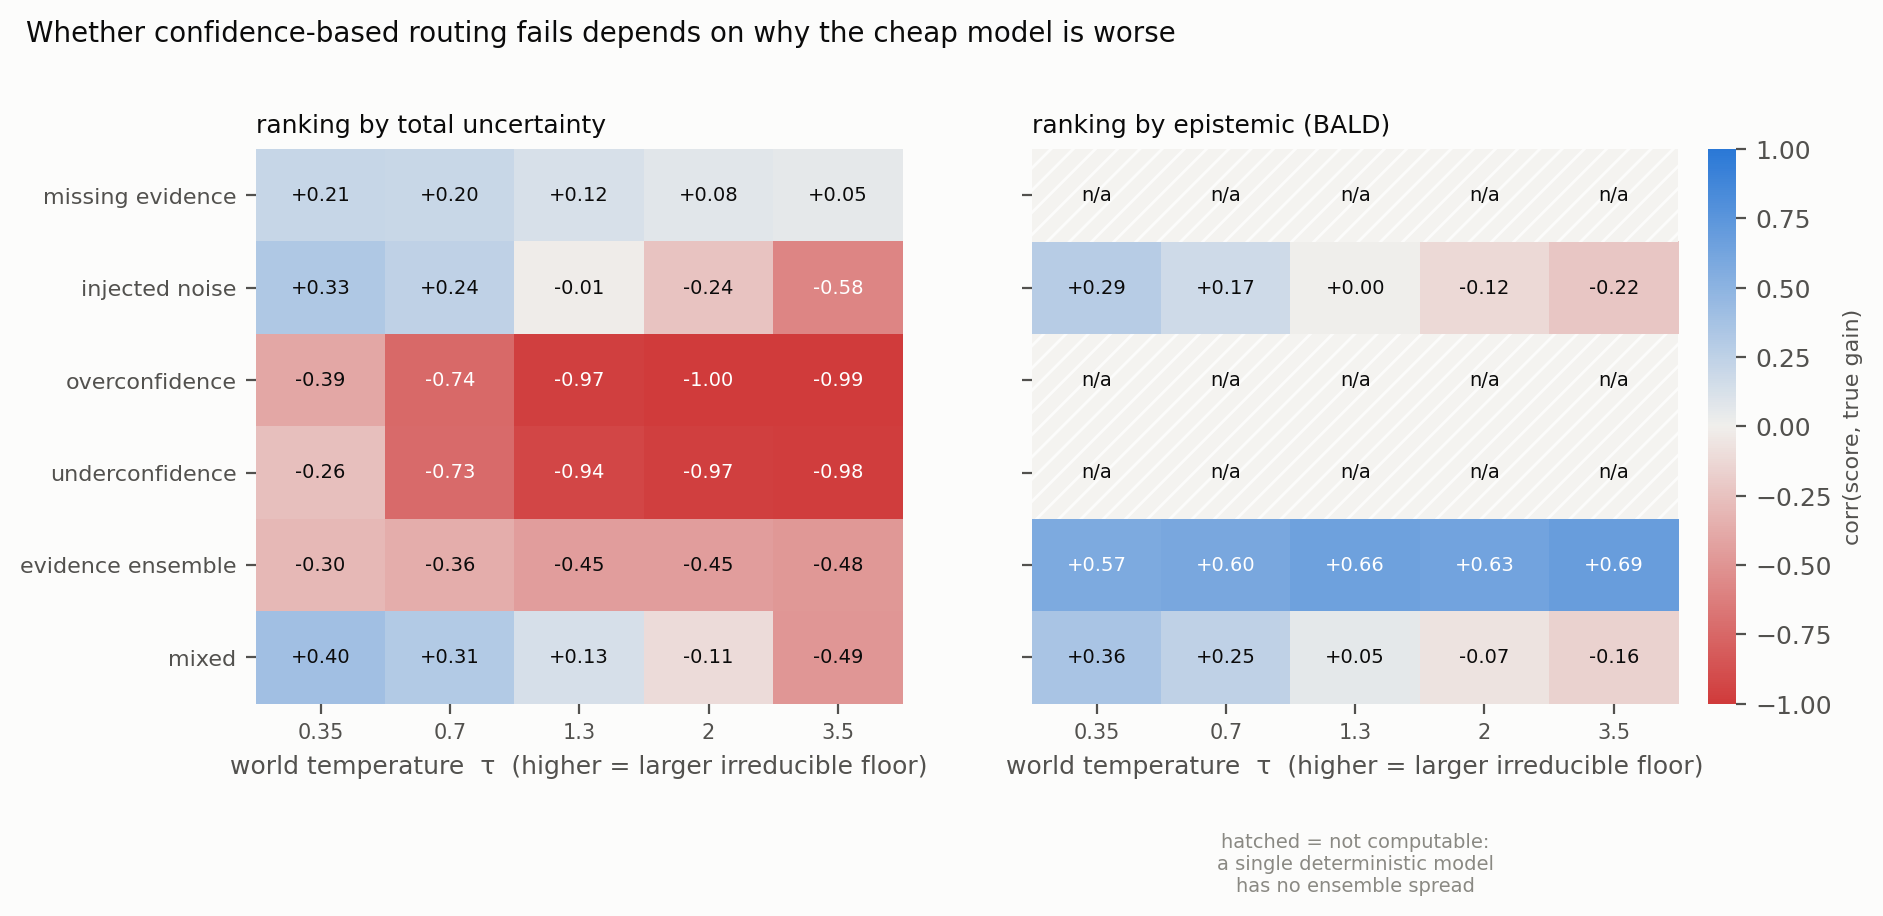
\includegraphics[width=\textwidth]{figures/fig4_mechanisms.png}
\caption{The mechanism map of Table~\ref{tab:mechanisms} as a heat map. Hatched cells are
configurations in which the estimate does not exist rather than being small.}
\label{fig:mechanisms}
\end{figure}

\FloatBarrier
\section{Budgeted curves and the skill score}
\label{app:curves}

The correlation reported throughout is a ranking diagnostic. The deployment-facing number is the
budgeted escalation curve: at budget $b$ the policy escalates the $b$ fraction of scenes it scores
highest, and the curve reports the resulting mean expected loss. Efficiency is normalised against
the oracle \emph{at the same budget}, since a policy at budget $b$ cannot do better than escalating
the $b$ scenes with the largest true gain, and then rescaled so that random routing scores $0$ and
the oracle $1$. Without that rescaling a random policy scores about $0.6$ against the oracle, which
compresses every comparison into the top of the range and makes a policy that is worse than random
still look as though it captures most of the gain.

% Generated by scripts/make_paper_tables.py -- do not edit.
The floor sweep with a single cheap/expensive pair, for reference, since it is the
setting in which the effect was first reported: ranking by total predictive uncertainty correlates
\RoutTotalLo{} with the true gain at the lowest floor and \RoutTotalHi{} at the highest, with a
budgeted skill of \RoutSkillTotalHi{} there --- that is, well below random. Ranking by the
epistemic estimate falls less far over the same sweep (\RoutBaldLo{} to \RoutBaldHi), and both pass
through zero near $\tau = 1.3$. \citet{peale2026flexible} report the same qualitative comparison
against a pointwise-optimal policy on synthetic data; what \S\ref{sec:mechanisms} adds is that
this setting is one row of a table whose other rows do not invert at all.

The correlation-sweep counterpart is in \S\ref{sec:confound}: the epistemic policy's budgeted
skill against random goes \RoutSkillBaldRhoZero{} at $\rho = 0$ to \RoutSkillBaldRhoHigh{} at
$\rho = 0.75$, so the budgeted number and the rank correlation agree about where the estimator
stops helping. Ties in a policy's scores are broken by index order rather than at random, which is
the pessimistic choice for a policy that emits many identical scores --- and that is the case worth
being pessimistic about, since a policy which cannot separate scenes should not be rewarded for it.


\FloatBarrier
\section{Robustness in full}
\label{app:robustness}

\begin{table}[h]
\centering
\small
\caption{Seed spread over \RobSeeds{} seeds, which re-draw the scenes and the forecasters' noise
streams, and the percentile bootstrap interval of the published run (\RobBoot{} resamples of the
scenes; the members are not a sample from a population, so they are not resampled). ``sign'' is
the fraction of seeds agreeing with the published sign.}
\label{tab:robustness}
\begin{tabular}{@{}p{0.33\textwidth}ccccc@{}}
\toprule
quantity & mean & sd & min, max & sign & bootstrap 95\% CI \\
\midrule
% Generated by scripts/make_paper_tables.py -- do not edit.
total unc.\ $\to$ gain, missing evidence, $\tau{=}3.5$ (junction) & \ensuremath{+0.025} & 0.019 & \ensuremath{+0.009}, \ensuremath{+0.046} & 100\% & [\ensuremath{-0.001}, \ensuremath{+0.086}] \\
total unc.\ $\to$ gain, overconfidence, $\tau{=}3.5$ (junction) & \ensuremath{-0.993} & 0.001 & \ensuremath{-0.993}, \ensuremath{-0.991} & 100\% & [\ensuremath{-0.994}, \ensuremath{-0.990}] \\
BALD $\to$ gain, evidence ensemble, $\tau{=}3.5$ (junction) & \ensuremath{+0.652} & 0.012 & \ensuremath{+0.638}, \ensuremath{+0.663} & 100\% & [\ensuremath{+0.630}, \ensuremath{+0.694}] \\
aleatoric share of prefix gain, $1\!\to\!2$ (junction) & 95\% & 0.007 & 94\%, 95\% & 100\% & --- \\
total unc.\ $\to$ prefix gain, $1\!\to\!2$ (junction) & \ensuremath{+0.145} & 0.008 & \ensuremath{+0.134}, \ensuremath{+0.156} & 100\% & --- \\
rise in KL$(P^*\|\bar Q)$, $\rho\!:\!0\to1$ (junction) & 10.3\ensuremath{\times} & 0.206 & 10.0\ensuremath{\times}, 10.6\ensuremath{\times} & 100\% & --- \\
total unc.\ $\to$ gain, missing evidence, $\tau{=}3.5$ (kitchen) & \ensuremath{+0.186} & 0.034 & \ensuremath{+0.135}, \ensuremath{+0.221} & 100\% & [\ensuremath{+0.127}, \ensuremath{+0.210}] \\
total unc.\ $\to$ gain, overconfidence, $\tau{=}3.5$ (kitchen) & \ensuremath{-1.000} & 0.000 & \ensuremath{-1.000}, \ensuremath{-1.000} & 100\% & [\ensuremath{-1.000}, \ensuremath{-1.000}] \\
BALD $\to$ gain, evidence ensemble, $\tau{=}3.5$ (kitchen) & \ensuremath{+0.840} & 0.007 & \ensuremath{+0.831}, \ensuremath{+0.849} & 100\% & [\ensuremath{+0.828}, \ensuremath{+0.858}] \\
aleatoric share of prefix gain, $1\!\to\!2$ (kitchen) & 97\% & 0.011 & 96\%, 98\% & 100\% & --- \\
total unc.\ $\to$ prefix gain, $1\!\to\!2$ (kitchen) & \ensuremath{+0.056} & 0.010 & \ensuremath{+0.046}, \ensuremath{+0.072} & 100\% & --- \\
rise in KL$(P^*\|\bar Q)$, $\rho\!:\!0\to1$ (kitchen) & 9.9\ensuremath{\times} & 0.077 & 9.8\ensuremath{\times}, 9.9\ensuremath{\times} & 100\% & ---
 \\
\bottomrule
\end{tabular}
\end{table}

\FloatBarrier
\section{Reproduction}
\label{app:repro}

Everything is CPU-only, single-process, and about ninety seconds end to end for the main results;
the seed sweep in Appendix~\ref{app:robustness} takes a few minutes more. There is no GPU, no
network access, no API key and no data file involved. Each experiment writes one row per scored
prediction alongside the reduced numbers, so every figure in this paper traces to the rows it came
from, and the paper's own numerals are generated from those files rather than typed.

% Generated by scripts/make_paper_tables.py -- do not edit.
\begin{verbatim}
python3 tests/test_instrument.py             # 23/23 identities
python3 scripts/validate_instrument.py       # 7/7 checks
python3 scripts/validate_instrument.py --world kitchen --tau 0.70
python3 scripts/run_decomposition.py         # Table 5
python3 scripts/run_routing.py               # Appendix D
python3 scripts/run_mechanisms.py            # Table 2
python3 scripts/run_mechanisms.py --world kitchen        # Table 6
python3 scripts/run_prefix.py                # Table 3
python3 scripts/run_prefix.py --world kitchen --tau 0.70
python3 scripts/run_robustness.py            # Table 7
python3 scripts/make_figures.py
python3 scripts/audit_numbers.py             # re-measures the docs
python3 scripts/make_paper_tables.py         # this paper's numbers
python3 scripts/audit_paper.py               # fails on any drift
\end{verbatim}

Results land in \texttt{experiments/results/<name>/} as a \texttt{records.csv} (one row per scored
prediction) and a \texttt{summary.json} (the reduced numbers), so every claim traces to the rows it
came from. Seeds derive from one root through a hash of a label path, so adding an arm to an
experiment cannot change the draws of the arms beside it.


\end{document}
